\begin{remark}
    Section made from lectures done by Jøran Moen. Other sources are \citet{BrekkeAsgeir2013Potu} --- chapter 3 parts 9, 12, 15 \& 16 ---, \citet{1995Itsp} --- chapter 13 parts 1 to 5 ---, \citet{NewellP.T.2004Mopb} and \citet{1992AnGeo..10..103C}.
\end{remark}
\section[High-latitude convection patterns \& field-aligned currents]{High-latitude convection patterns and field-aligned currents (AB 3.16)}
\Cref{fig:L13_high_latitude_flow} show an idealized representation of the plasma flow in the high-latitude and polar cap ionosphere. This has a symmetric two-cell system with clockwise rotation on the dusk side and anticlockwise rotation on the dawn side. Plasma convection is thought to be driven by the dawn-dusk electric field \(\gf{E}_{pc}\) across the polar cap. The return flow takes place along narrow belts at lower latitudes in the auroral oval. The points \(P\) and \(Q\) are related to high and low potentials, respectively, thus a poleward electric field, \(\gf{E}_a\), occurs on the dusk side and an equatorward electric field on the dawn side of the auroral oval, respectively.

Flow reversal takes place at about \SI{70}{\degree} to \SI{80}{\degree} of latitude on the dawn/dusk sides. Since rotation is clockwise in the dawn sector at \(P\), a positive potential takes place here, while the opposite is true on the dusk side at \(Q\).
\begin{figure}[t]
    \centering
    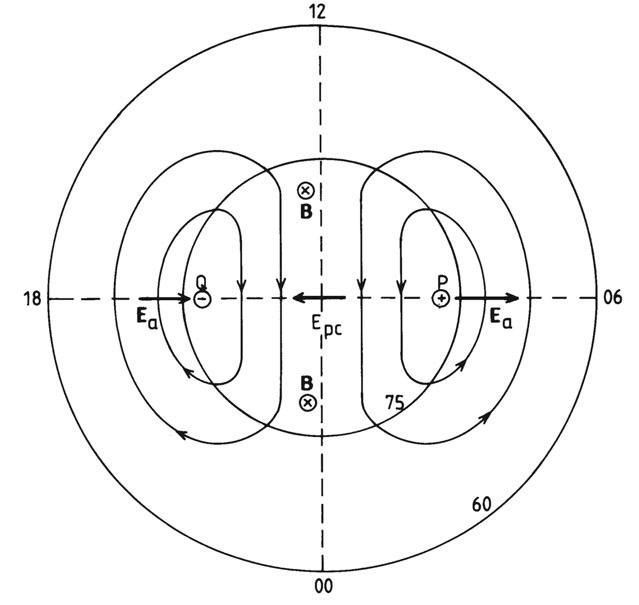
\includegraphics[width=.6\linewidth]{bilder/L13_high_latitude_flow.jpg}
    \caption{Simplified model of the high latitude ionospheric convection pattern showing a symmetric two-cell system with clockwise rotation on the dusk side and anticlockwise rotation on the dawn side.}\label{fig:L13_high_latitude_flow}
\end{figure}

A result which has emerged from satellite measurements is the presence of field-aligned currents at any time. A sketch of this pattern can be found in \cref{fig:L13_field_aligned_currents}. It show the currents for IMF southward, and the currents into and out of the ionosphere are indicated by different symbols, thus showing currents out of the ionosphere in the evening and into the ionosphere in the morning associated with the region-1 current. The equatorial currents that enter the ionosphere in the evening and leave the ionosphere in the morning are associated with region-2 currents. The field-aligned currents at very high latitude at noon (cusp currents) are strongly dependent on the \(B_y\)-component of the IMF\@.

To better our understanding of the dawn-dusk current system between the ionosphere and magnetosphere, we look to the diagram in \cref{fig:L13_polar_cap_currents}. Here, the Earth is seen from the nightside with the midnight meridian marked as the diameter. The field-aligned currents in the dawn-dusk meridian are in accordance with the satellite observations. In the ionosphere we know that the auroral zone electric field \(\gf{E}_a\) is directed northward in the dusk sector and southward in the dawn sector (dusk to dawn). Since the ionosphere has finite conductivity, the field-aligned currents will mainly shorten in the ionosphere as a result of Pedersen currents, northward in the dusk sector and southward in the dawn sector. The closure of the loop in the magnetosphere is not well established, but we here let it be radial in the dusk-dawn direction. These are currents closing between \(Q'\) and \(Q''\), and \(P'\) and \(P''\). We notice that when the dusk-dawn auroral zone electric field is mapped out to the magnetosphere, they will be reversed and directed from dawn to dusk in agreement with the polar cap and cross-tail electric fields \(\gf{E}_{pc}\) and \(\gf{E}_m\), respectively. In the magnetosphere the electric field and currents are antiparallel and thus form a generator, while they are parallel in the ionospheric load.
\begin{figure}[t]
    \centering
    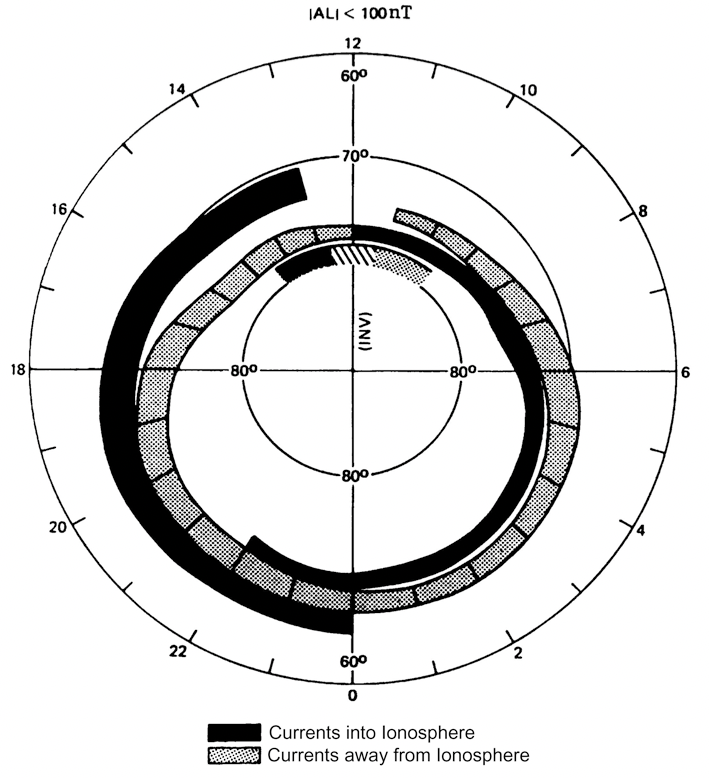
\includegraphics[width=.6\linewidth]{bilder/L13_field_aligned_currents.png}
    \caption{The average pattern of field-aligned currents in the high-latitude region when the IMF is southward. (From Ijiima and Potemra, 1976.)}\label{fig:L13_field_aligned_currents}
\end{figure}
\begin{figure}[t]
    \centering
    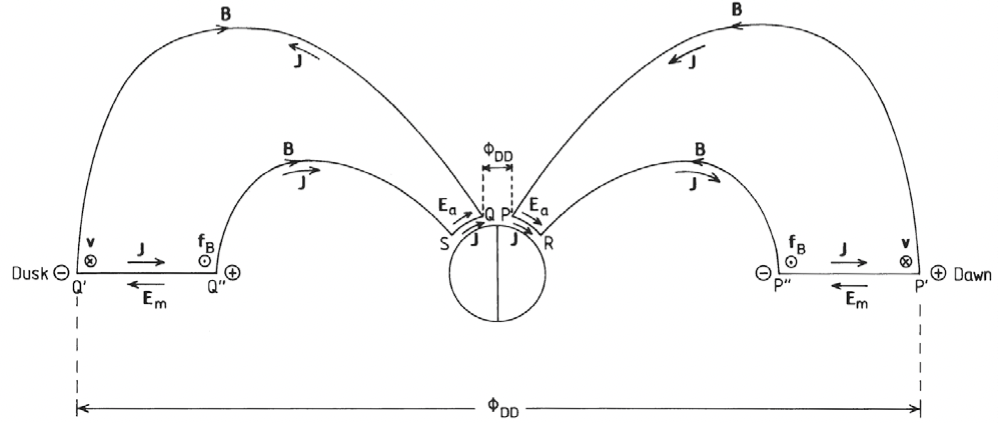
\includegraphics[width=.9\linewidth]{bilder/L13_polar_cap_currents.png}
    \caption{Possible synthesis of ground-based and satellite observations of the ionospheric-magnetospheric current system and electric fields. The cross-section is in the \(y\)--\(z\)-plane along the dawn-dusk meridian seen from the tail side of the Earth (toward the Sun). The magnetospheric dynamo drives the currents in the dusk-dawn direction in the ecliptic plane. These currents continue to the ionosphere as currents parallel to \(B\). In the ionosphere they are deflected in the horizontal direction as Pedersen currents along the auroral zone electric field. The magnetic force \(\gf{f}_B\) in the ecliptic plane opposes the convection velocity \(\gf{v}\). The electric potential \(\phi_{DD}\) in the magnetosphere between the dawn and the dusk sector is projected along the magnetic field line across the polar cap between the points \(P\) and \(Q\) on the dawn and dusk side, respectively.}\label{fig:L13_polar_cap_currents}
\end{figure}

\section[Types of magnetic activity]{Types of magnetic activity (K\&R 13.2)}
An important prerequisite for this section is the coordinate system in \cref{fig:magnetometer_coor}.
\subsection{Magnetospheric substorms}
The most frequent type of activity is referred to as a magnetospheric substorm. A substorm is the ordered sequence of events that occurs in the magnetosphere and ionosphere when the IMF turns southward and increased energy flows from the solar wind into the magnetosphere. The most obvious manifestation of a substorm is the aurora, and during substorms, quiet auroral arcs suddenly explode into brilliance.

Magnetic disturbances come with these auroras, and on the ground beneath the aurora, magnetometers will record intense disturbances caused by electric currents in the ionosphere. Stations located in the afternoon-to-evening sector record positive disturbances in the \(H\)-component of the magnetometers, while stations near the past midnight record negative disturbances. From this we deduce that the currents causing the disturbances flow eastward and westward, respectively, and these currents are called the electrojets. From the magnetometer readings we get the AE index.
\begin{equation*}
    AE=AL-AU
\end{equation*}
meaning the envelope of the negative disturbances minus the envelope of the positive disturbances.

\subsection{Magnetic storms}
When coupling of the solar wind to the magnetosphere becomes strong and prolonged and geomagnetic activity becomes intense, a magnetic storm will develop. During the storm, the auroral currents are almost continuously disturbed, and the development of the storm is best seen at mid-latitudes in the \(D_{st}\) index. This index is based on the \(H\)-component of 6 magnetometers around equator, measuring the ring current, a current created by particles drifting in the Van Allen radiation belts at 3--5\(R_E\). A plot of the \(D_{st}\) index is shown in \cref{fig:L13_dst_index}.

A storm often begins with a sudden increase in magnetic field that may last for many hours. This initial phase is followed by a rapid and sometimes highly disturbed decrease in \(D_{st}\). This is the main phase of the storm. Subsequently the \(D_{st}\) begins a rapid recovery, the first stage of the recovery phase. Eventually, a stage of long, slow recovery ensues. The length of such a storm is often 1--5 days.
\begin{figure}[t]
    \centering
    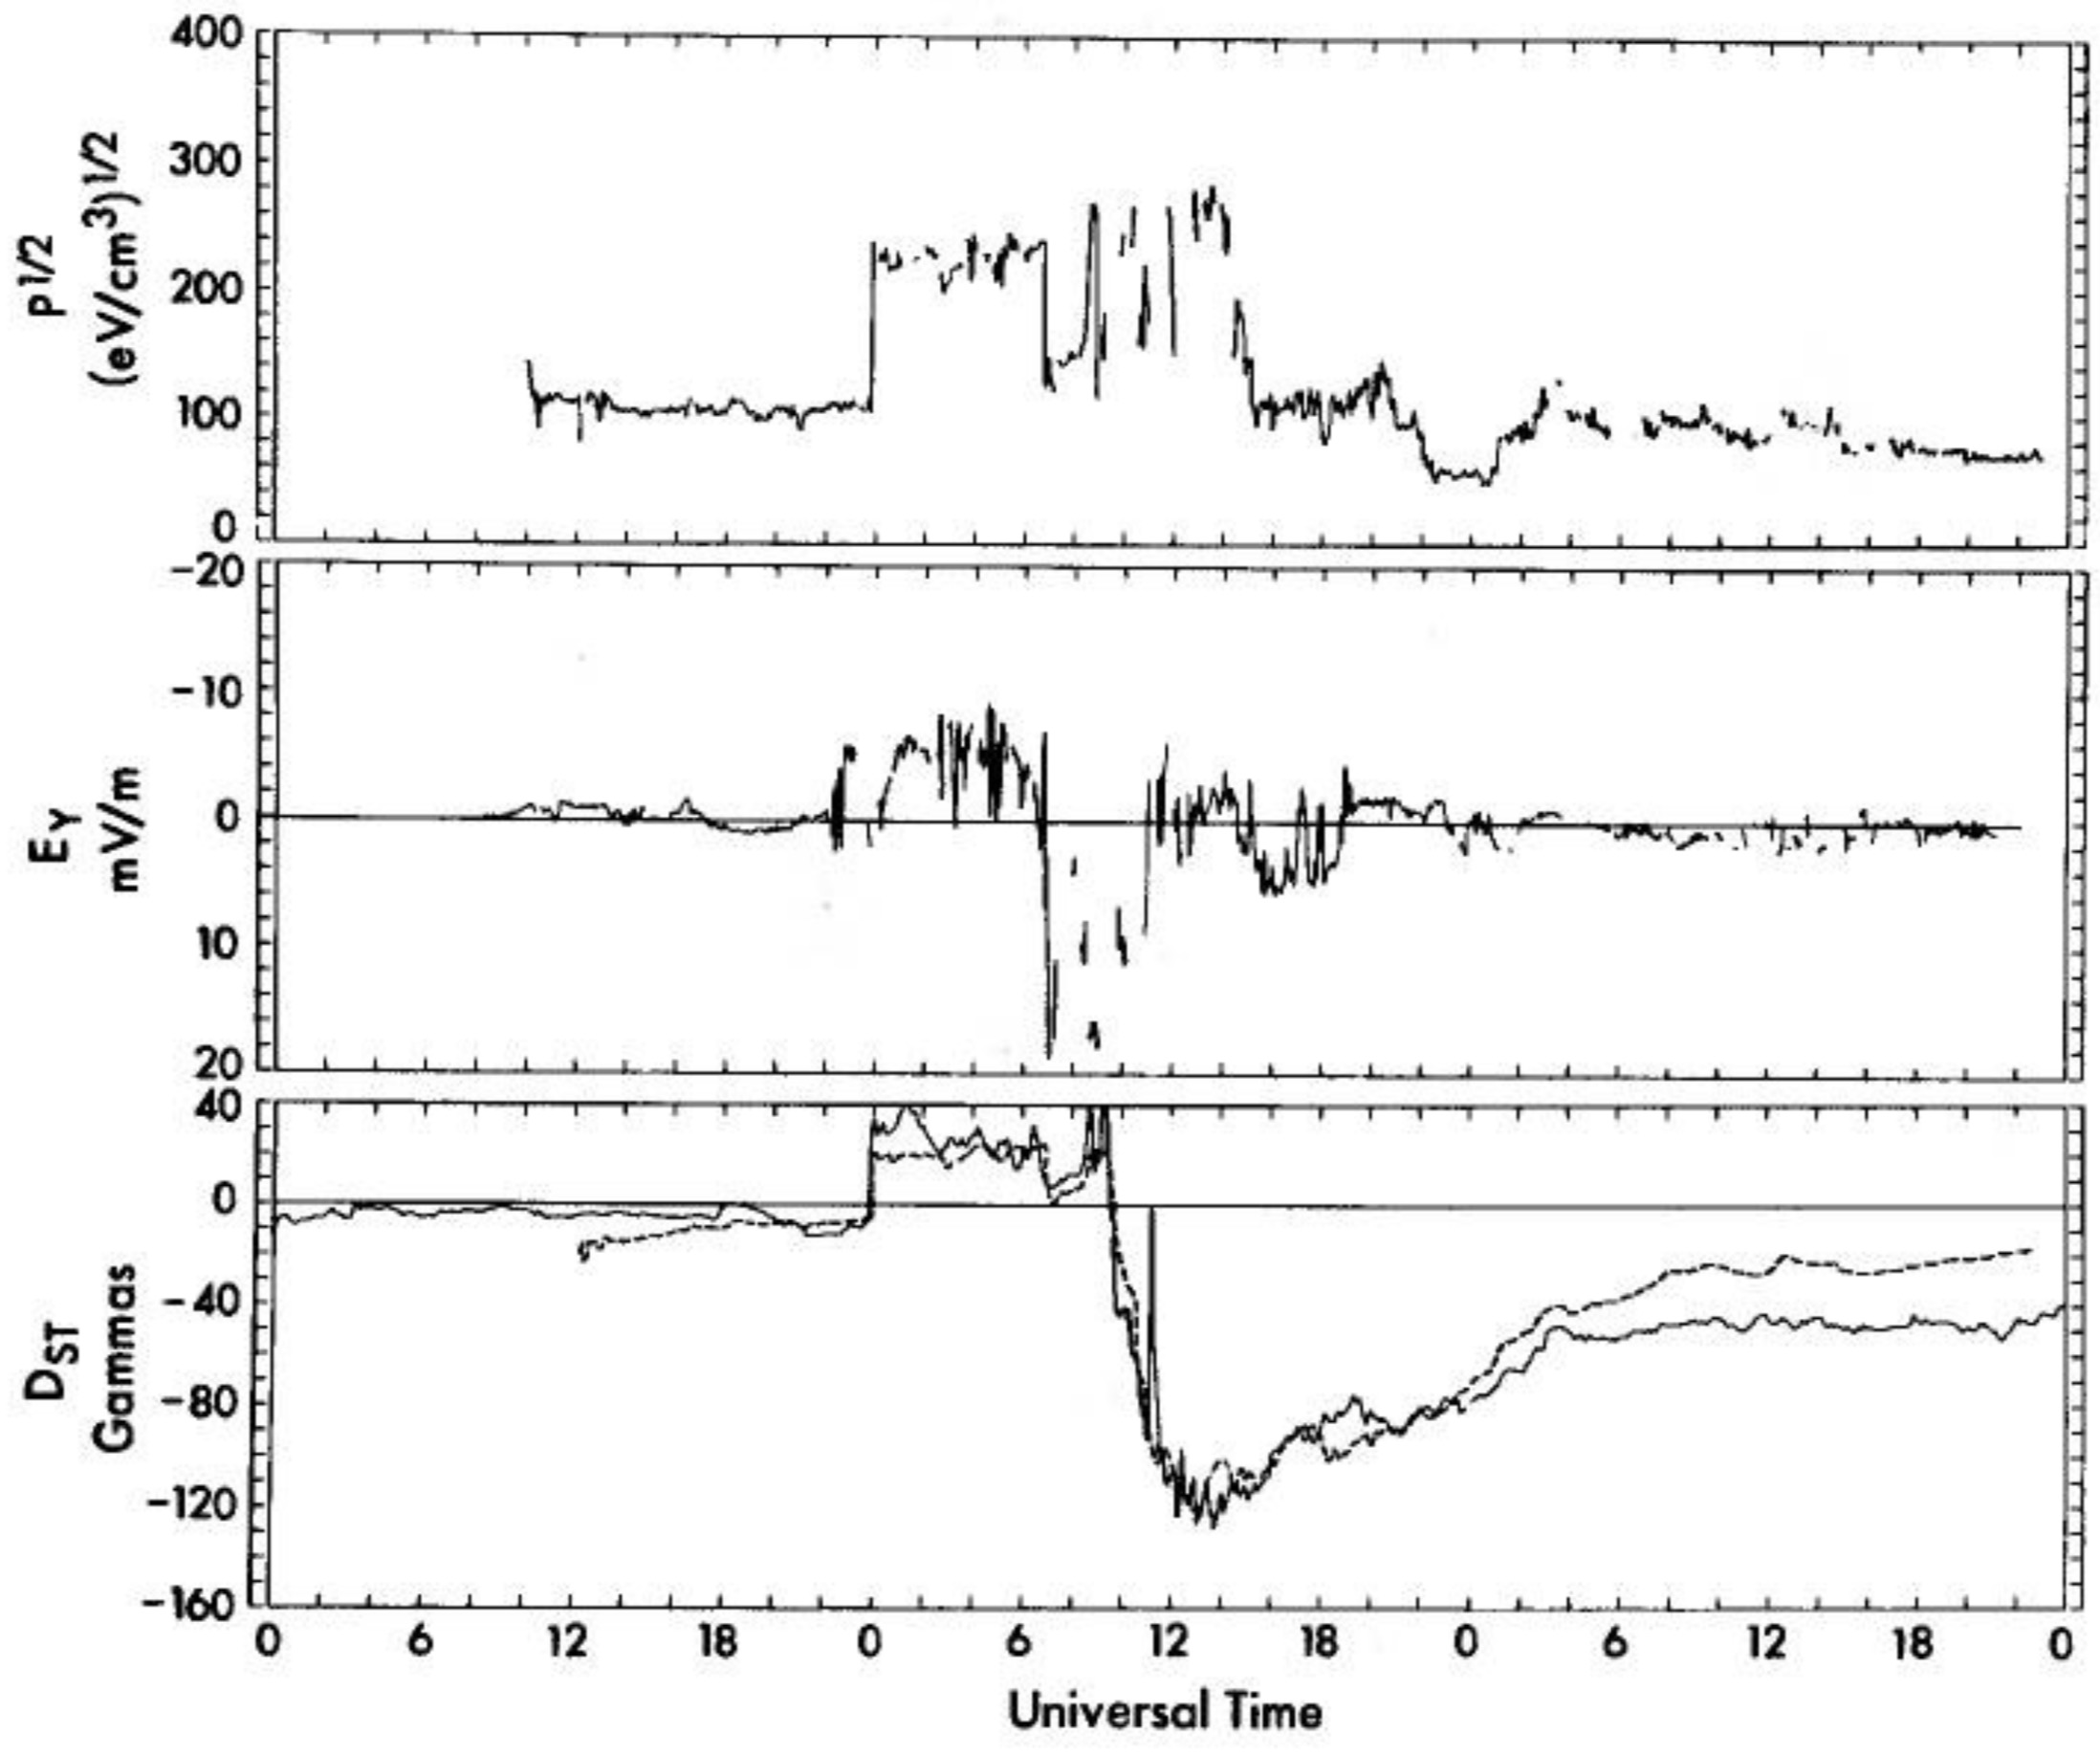
\includegraphics[width=.6\linewidth]{bilder/L13_dst_index.jpg}
    \caption{Measurement of solar wind and magnetic field on the surface of the Earth on 15--17 February 1967. Top: Solar-wind dynamic pressure. Middle: Dusk-to-dawn component of solar-wind electric field. Note that negative values of \(E_y\) are plotted upwards. Bottom: Effects of a magnetic storm as recorded in the \(D_{st}\) index. (From Burton et al. 1975.)}\label{fig:L13_dst_index}
\end{figure}

\section[Signatures of tail reconnection]{Signatures of tail reconnection (C\&L)}
The signatures in the 6300 Å MSP keogram is a good proxy for tail reconnection.

Studies of ionospheric flow and their relation to interplanetary conditions began using electric fields, plasma drift and magnetic reconnection. From magnetic observations from the ground, the existence of three important effects was demonstrated. (1) For much of the time the flows at high-latitudes are of two-cell form. Also, the flow system is larger and stronger when IMF \(B_z\) is negative compared to when it is positive. (2) The two-cell flow also exhibits a number of dawn-dusk asymmetries, largely dependant on \(B_y\). (3) Occasionally, sunward-directed flows are observed in the central polar cap which are indicative of multi-cell (often three) convection cells. These types of multi-cells are typical for ``significantly'' northward IMF \(B_z\). The three effects can be understood, firstly from the modulation of the flow by the IMF \(B_z\), and the amount of open flux which the system contains. Second, when new flux is opened the east-west tension it experiences may lead to asymmetries, and third, flow effects in the central flow cell under IMF \(B_z\) positive are believed to result from reconnection between the IMF and pre-existing open flux in the tail lobe.

The flow pattern cannot be modeled only by one single parameter, the IMF vector, but to make simple but meaningful models, two parameters, IMF and tail processes, suffices. The parameter taking care of tail processes is often related to the past history of the interplanetary medium and magnetosphere in a more complex manner.

The form of the ionospheric flow due to only dayside reconnection can be seen in the sketch in \cref{fig:L13_dayside_tail_reconnection_only}, \textbf{a}. Effects of \(B_y\) is not implemented. The plasma flow crosses the boundary only across the dashed line, making the polar cap expand. In \textbf{b} the same kind of sketch is made for unbalanced tail reconnection, where we see the polar cap contract. If we let the voltage across the dashed line be \(V\) in \textbf{a}, then it decreases to about \(V/2\) across the center of the polar cap, and then to zero by the nightside boarder. Only when the flow is the same in and out you get a voltage of \(V\) at all positions poleward of the merging gaps.
\begin{figure}[t]
    \centering
    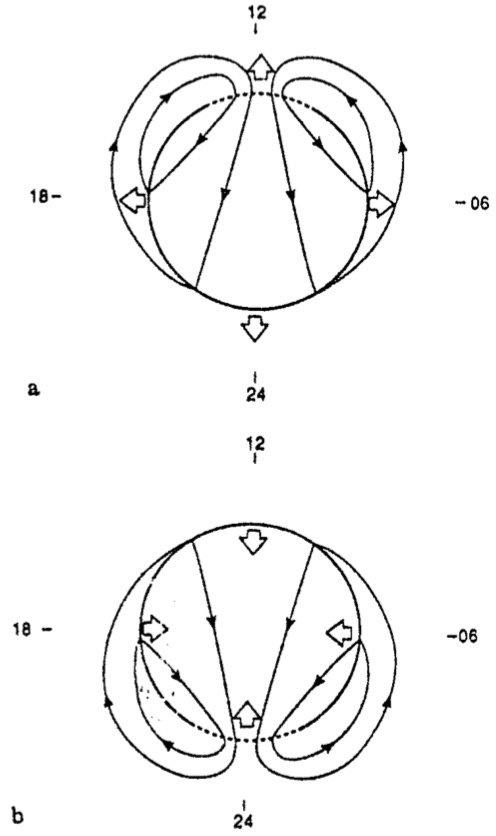
\includegraphics[width=.4\linewidth]{bilder/L13_dayside_tail_reconnection_only.jpg}
    \caption{Sketch showing the form of the two basic time-dependant components of the high-latitude ionospheric flow due to \textbf{a} unbalanced reconnection on the dayside and \textbf{b} unbalanced reconnection in the tail.}\label{fig:L13_dayside_tail_reconnection_only}
\end{figure}

Since the rate of tail reconnection lags behind the dayside reconnection, we might want to add a delay. The delay arises from the finite information propagation speed between the subsolar region where dayside reconnection occurs and the reconnection region in the tail. The information propagation speed will be a few hundred km/s, and then if the neutral line lies downtail at about 100--150 \(R_E\), the information delay will be 20--30 min. Furthermore, when the response has occurred, the information will propagate back to the ionosphere at a speed corresponding to the Alfv\'{e}n speed in the tail lobes (1000 km/s), adding an extra delay of at least 10 min.

With an estimate of 30 min delay time, and in a situation where we have \(B_z\) positive, only interrupted by 1 hour of \(B_z\) negative, we will see the change in voltage as plotted in \cref{fig:L13_voltage_dependance_flux_flow}. Across the dayside boarder the voltage goes from 0 to \(V\) once reconnection starts, while the same is true on the nightside after a delay time of 30 min. The total open flux is presented in the next panel, \textbf{d}, and then, with a least squares average we get the voltage across the central polar cap, going from 0 when there is no flow, to \(V/2\) when only one reconnection process is going and \(V\) when we have reconnection on both sides. The polar cap voltage also includes the effect of the additional propagation delay from the reconnection regions to the ionosphere, and the finite time scale for system response (15 min).
\begin{figure}[t]
    \centering
    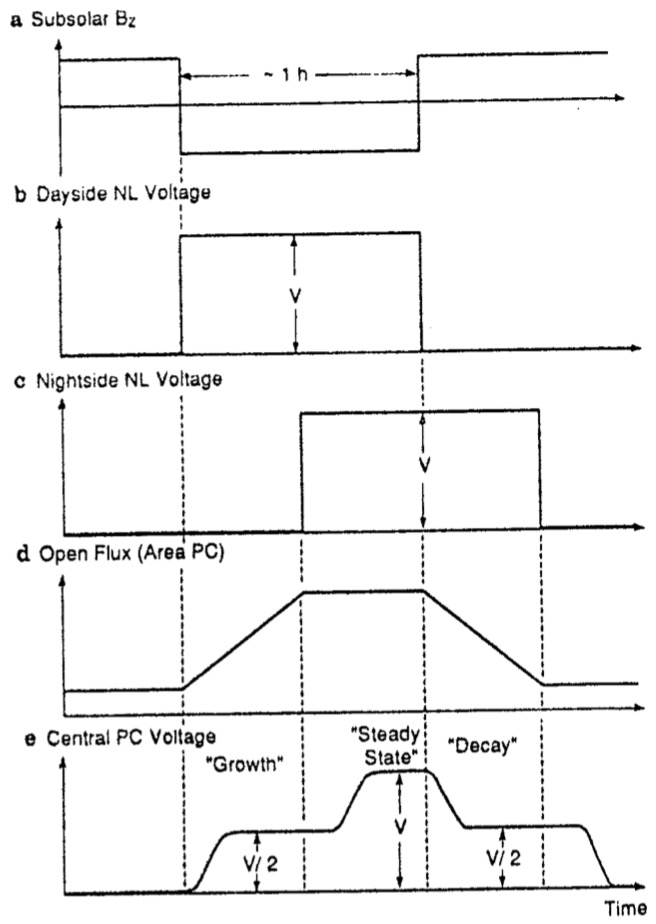
\includegraphics[width=.4\linewidth]{bilder/L13_voltage_dependance_flux_flow.jpg}
    \caption{Sketch of how the voltage and flux changes on the dayside and nightside for an idealized situation with one hour of \(B_z\) negative, positive otherwise.}\label{fig:L13_voltage_dependance_flux_flow}
\end{figure}

Different flow patterns may appear, and if we consider for a moment a completely closed polar cap, we may then introduce a change in flux on the dayside, \(\tn{d}F\), to give a crude model of different flows. With \(B_y=0\) we will get extra flux at noon, and the two-cell pattern appears. If, on the other hand, we had \(B_y\) positive, East-West tension force would drag the extra flux over towards the dawn side, as sketched in \cref{fig:L13_flow_from_positive_By}. The opposite will of course hold for \(B_y\) negative.
\begin{figure}[t]
    \centering
    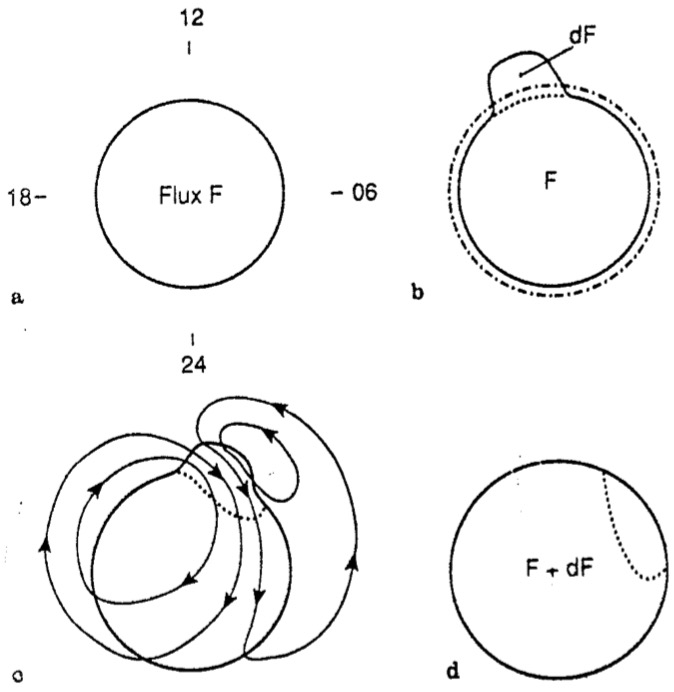
\includegraphics[width=.4\linewidth]{bilder/L13_flow_from_positive_By.jpg}
    \caption{Sketch of how the flow pattern will look like for both \(B_z\) and \(B_y\) positive and no reconnection on the nightside.}\label{fig:L13_flow_from_positive_By}
\end{figure}

More complicated and unpredictable flows can appear during \(B_z\) positive, where the flows, insteas of being driven by dayside reconnection, are driven by ``viscous'' processes. A typical feature is a circular cell in the middle of the polar cap.

From this discussion, we can easily understand that the OCB moves northward when we get reconnection in the tail, and that reconnection on the dayside will immediately transfer to the nightside, expanding the auroral oval and pushing the OCB equatorward. On the dayside, when you reconnect, you go from a closed loop to an open loop, i.e.\ you have open magnetic flux. On the nightside, it is the open field lines that is closing, and you have a closing magnetic flux. On the dayside you get an excess of plasma, while on the nightside you loose some plasma. In between the filled lines and the plasma is frozen into each other, i.e.\ we have an adiaroic boundary.

\section{Precipitation patterns}
When talking about reconnection and the expansion and contraction of the polar cap, it might be nice to take a revisit to the precipitation pattern. Referring to \cref{fig:L4_maps_precipitation_pattern}, we add to this image what is sketched in \cref{fig:L13_regions_of_precipitation}. The nighttime aurora come from the PSBL with energies at \(1\)--\(20\) keV. The energies in the LLBL/cusp/mantle is \(<1\) keV, while for the CPS we find \(>20\) keV.
\begin{figure}[t]
    \centering
    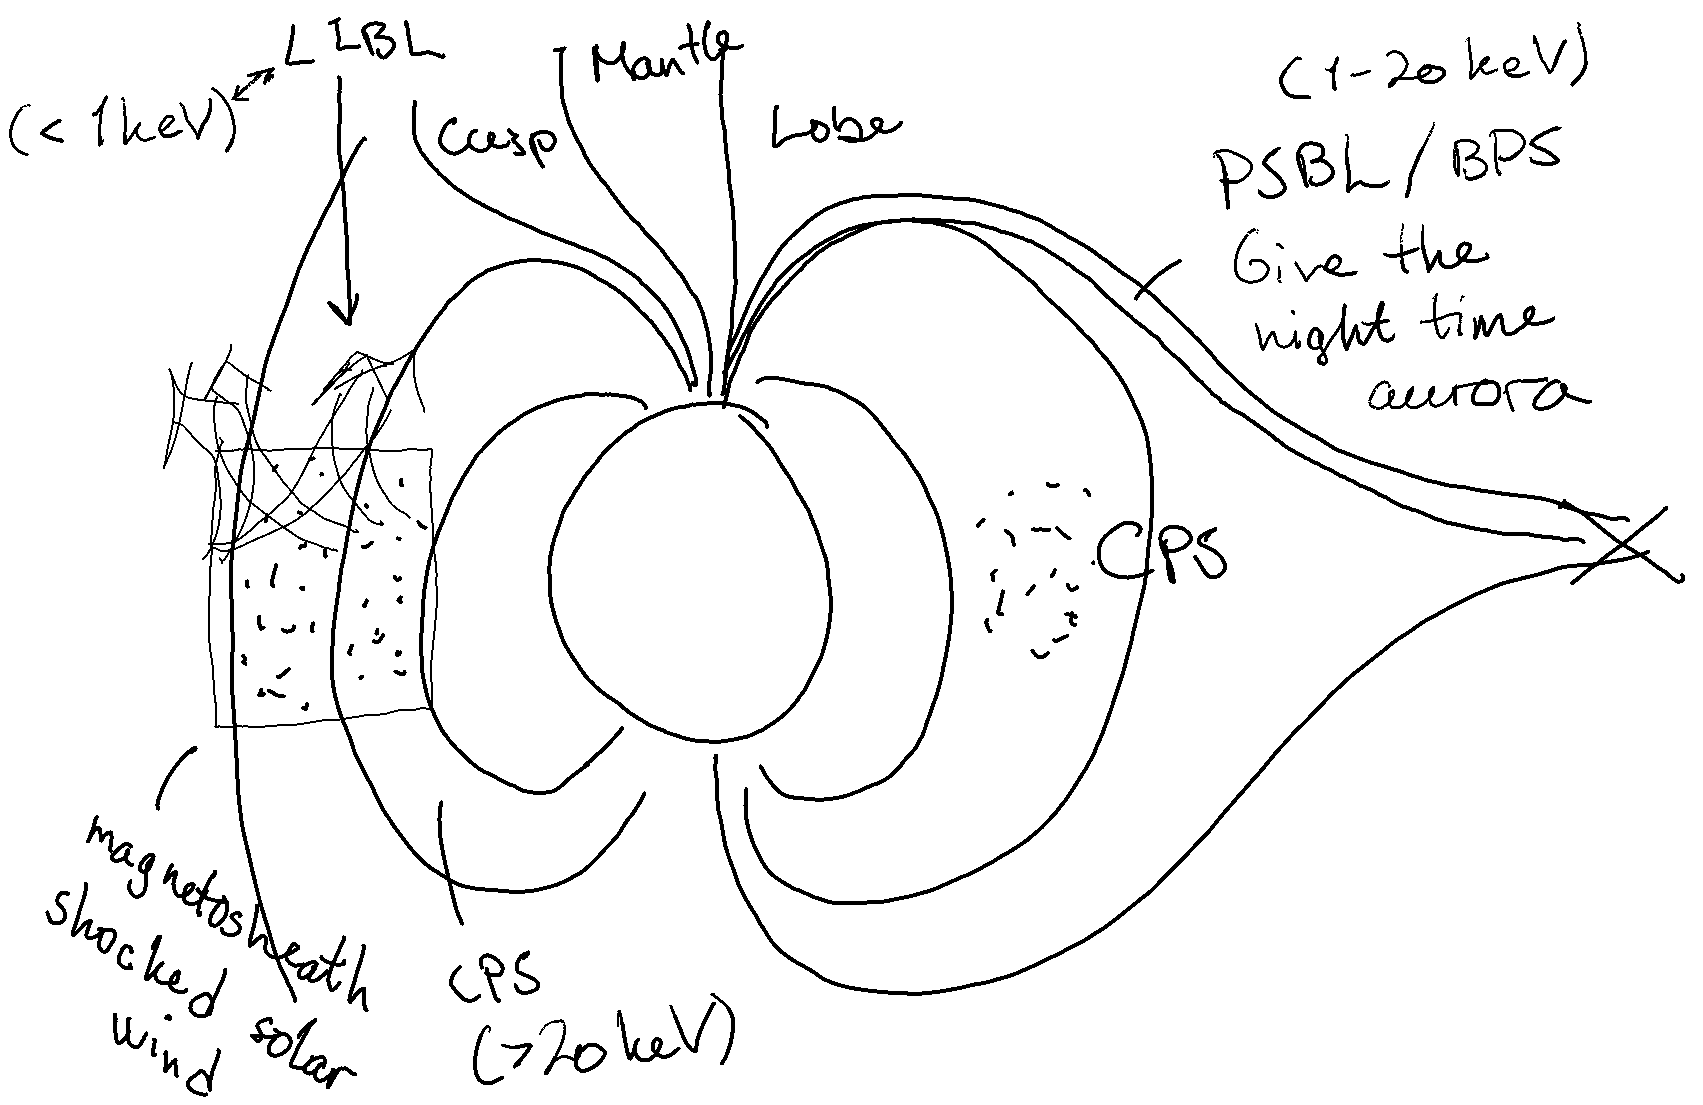
\includegraphics[width=.8\linewidth]{bilder/L13_regions_of_precipitation.png}
    \caption{Sketch showing the different precipitation regions see in the \(y=0\) plane, in negative \(y\)-direction.}\label{fig:L13_regions_of_precipitation}
\end{figure}
